\chapter*{Úvod}
\phantomsection
\addcontentsline{toc}{chapter}{Úvod}

V dnešní době jsou sítě IoT téměř na každém kroku. Proto se snaží i~velcí výrobci domácí elektroniky implementovat tuto konektivitu do svých zařízení. Většinou se jedná o~uzavřený ekosystém senzorů, které spolu komunikují pomocí sítě využívající bezlicenční pásma a~přenáší data na server, kde se dále zpracovávají a~vyhodnocují. Lze je tedy dnes najít v~mnoha rodinách, kde se mohou zapojit do chytré domácnosti, či mnohem častěji v~průmyslu při automatizaci výrobních procesů.

V komerčním prostředí nejsou zatím dostupná žádná zařízení, která by umožňovala monitorovat kvalitu ovzduší v~domácích podmínkách. Lze nalézt mnoho profesionálních zařízení, které jsou určeny na měření jedné konkrétní veličiny (např. koncentrace prachových částic), avšak takové zařízení stojí tisíce korun. Cílem této práce je navrhnout, oživit a~naprogramovat zařízení, které umožní monitorovat a~vyhodnocovat základní veličiny o~kvalitě ovzduší.

Základní myšlenkou IoT sítí a~zařízení do nich připojených je velice nízká spotřeba, díky čemuž dokáží vydržet v~provozu na baterie i~několik let. Nízké spotřeby je dosaženo nejen vybranými senzory a~řídícím mikroprocesorem, ale hlavně díky nízkým nárokům na počet přenesených dat a~vysílací výkon. Celé zařízení tedy bude navrhováno s~ohledem na výslednou spotřebu při zachování uspokojivé přesnosti měření a~také ceně použitých komponent.

Výsledky měření budou přenášeny do databáze, odkud se mohou používat pro vykreslování do grafů či pro následné zpracování ve formě rychlých přehledů (např. průměrné denní hodnoty). Tyto výsledky budou předávány uživateli skrze webovou službu, takže si je bude moci zobrazit v~podstatě na jakémkoli zařízení, které je připojeno k~internetu. Blokové schéma popisující fungování zařízení lze vidět na obrázku \ref{fig_BlockDiagram-blank}.

\begin{figure}[h]
    \centering
    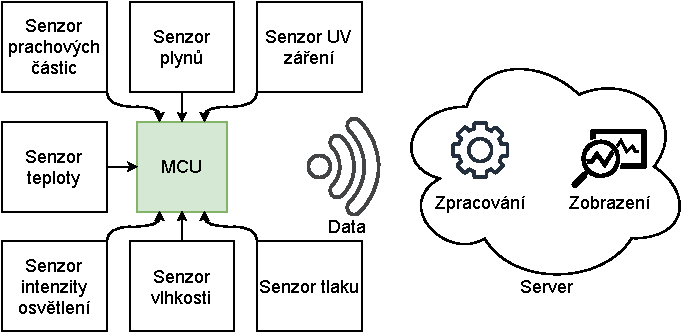
\includegraphics{obrazky/block_schematic-blank.drawio.pdf}
    \caption{Blokový diagram výsledné funkce zařízení.}
    \label{fig_BlockDiagram-blank}
\end{figure}